% !TeX root = main.tex

\chapter{Fast Fourier Transform}
\glsresetall
\label{chapter:fft}

Performing the \gls{dft} directly using matrix-vector multiply requires $\mathcal{O}(n^2)$ multiply and add operations for an input signal with $n$ samples.  It is possible to reduce the complexity by exploiting the structure of the constant coefficients in the matrix.  This $S$ matrix encodes the coefficients of the \gls{dft}; each row of this matrix corresponds to a fixed number of rotations around the complex unit circle (please refer to Chapter \ref{sec:DFTbackground} for more detailed information). These values have a significant amount of redundancy, which can be exploited to reduce the algorithm's complexity. 

\begin{aside}
The 'Big O' notation used here describes the general order of an algorithm's complexity based on the input data's size.  For a complete description of Big O notation and its use in analyzing algorithms, see \cite{CLR}.
\end{aside}

The \gls{fft} uses a divide-and-conquer approach based on the symmetry of the $S$ matrix.  The \gls{fft} was made popular by the Cooley-Tukey algorithm \cite{cooley65}, which requires $\mathcal{O}(n \log n)$ operations to compute the same function as the \gls{dft}.  This can provide a substantial speedup, especially when performing the Fourier transform on large signals. %Other optimizations are also possible based on the fact that each element of the $S$ matrix has magnitude '1'.  We will mention some of these optimizations, but generally focus on the architectural tradeoffs in implementing the \gls{fft}.

\begin{aside}
Karl Friedrich Gauss initially developed the divide-and-conquer approach to computing the \gls{dft} in the early 19th century. However, since Gauss' work on this was not published during his lifetime and only appeared after his death, it was relegated to obscurity.  Heideman et al.~\cite{heideman84} provide an excellent background on the history of the \gls{fft}.
\end{aside}

The focus of this chapter is to provide the reader with a good understanding of the \gls{fft} algorithm since that is an important part of creating an optimized hardware design. Thus, we start by giving a mathematical treatment of the \gls{fft}. This discussion focuses on small \gls{fft} sizes to provide basic intuition on the core ideas. After that, we focus on different hardware implementation strategies.

\section{Background}

The \gls{fft} reduces complexity by taking advantage of symmetries in the \gls{dft} calculation. To better understand how to do this, let us look at \gls{dft} with a small number of points, starting with the 2 point \gls{dft}.  Recall that the \gls{dft} performs a matrix vector multiplication, i.e., $G[] = S[][] \cdot g[]$, where $g[]$ is the input data, $G[]$ is the frequency domain output data, and $S[][]$ are the \gls{dft} coefficients. We follow the same notation for the coefficient matrix and the input and output vectors as described in Chapter \ref{sec:DFTbackground}.

For a 2 point \gls{dft}, the values of $S$ are:
\begin{equation}
S =
 \begin{bmatrix}
  W^{0 0}_2 & W^{0 1}_2  \\
  W^{1 0}_2 & W^{1 1}_2 \\
 \end{bmatrix}
 \end{equation}
Here we use the notation $W = e^{-j 2 \pi}$. The superscript on $W$ denotes values added to the numerator, and the subscript on the $W$ indicates those values added to the denominator of the complex exponential. For example, $W^{2 3}_4 = e^{\frac{-j 2 \pi \cdot 2 \cdot 3}{4}}$. This is similar to the $s$ value used in the \gls{dft} discussion (Chapter \ref{sec:DFTbackground}) where $s = e^{\frac{-j 2 \pi}{N}}$. The relationship between $s$ and $W$ is $s = W_N$.

\begin{aside}
The $e^{-j 2 \pi}$ or $W$ terms are often called \term{twiddle factors}. This term has its origin in the 1966 paper by Gentleman and Sande \cite{gentleman1966fast}.
\end{aside}

\begin{equation}
\begin{bmatrix} 
G[0] \\ 
G[1] \\
\end{bmatrix} = 
 \begin{bmatrix}
  W^{0 0}_2 & W^{0 1}_2  \\
  W^{1 0}_2 & W^{1 1}_2 \\
 \end{bmatrix}
 \cdot
  \begin{bmatrix}
  g[0] \\
  g[1]\\
\end{bmatrix}
\end{equation}

Expanding the two equations for a 2 point \gls{dft} gives us:
\begin{equation}
\begin{array} {lll} 
G[0] & = & g[0] \cdot e^{\frac{-j 2 \pi \cdot 0 \cdot 0}{2}} + g[1] \cdot e^{\frac{-j 2 \pi \cdot 0 \cdot 1}{2}} \\
 & = & g[0] + g[1] \\
\end{array}
\label{eq:2ptlower}
\end{equation} due to the fact that since  $e^{0}  =  1$. The second frequency term
\begin{equation}
\begin{array} {lll} 
G[1] & = & g[0] \cdot e^{\frac{-j 2 \pi \cdot 1 \cdot 0}{2}} + g[1] \cdot e^{\frac{-j 2 \pi \cdot 1 \cdot 1}{2}} \\
 & = & g[0] - g[1] \\
\end{array}
\label{eq:2pthigher}
\end{equation} since  $e^{\frac{-j 2 \pi \cdot 1 \cdot 1}{2}}  = e^{-j \pi } = -1$.

Figure \ref{fig:2pointFFT} provides two different representations for this computation.  Part a) is the data flow graph for the 2 point \gls{dft}. It is the familiar view we have used to represent computation throughout this book. Part b) shows a butterfly structure for the same computation. This is a typical structure used in digital signal processing, in particular, to represent the computations in an \gls{fft}. 

The butterfly structure is a more compact representation of large data flow graphs. When two lines come together, an additional operation is performed. Any label on the line indicates a multiplication of that label by the value on that line. There are two labels in this figure. The `$-$' sign on the bottom horizontal line indicates that this value should be negated. This, followed by the addition denoted by the two lines intersecting, is the same as subtraction. The second label is $W^0_2$. While this multiplication is unnecessary (since $W^0_2 = 1$, this means it is multiplying by the value `$1$'), we show it here since it is a common structure that appears in higher point \gls{fft}s.

\begin{figure}
\centering
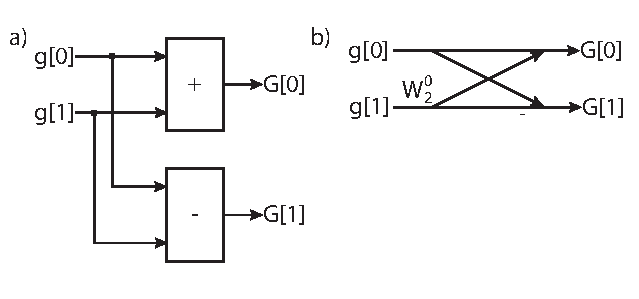
\includegraphics[width= 0.8 \textwidth]{images/2pointFFT}
\caption{Part a) is a data flow graph for a 2 point \gls{dft}/\gls{fft}. Part b) shows the same computation but shown as a butterfly structure. This is a common representation for the computation of an \gls{fft} in the digital signal processing domain.}
\label{fig:2pointFFT}
\end{figure}

Now let us consider a slightly larger \gls{dft} -- a 4 point \gls{dft}, i.e., one with 4 inputs, 4 outputs, and a $4 \times 4$ $S$ matrix. The values of $S$ for a 4 point \gls{dft} are:
\begin{equation}
S =
 \begin{bmatrix}
  W^{0 0}_4 & W^{0 1}_4 & W^{0 2}_4 & W^{0 3}_4 \\
  W^{1 0}_4 & W^{1 1}_4 & W^{1 2}_4 & W^{1 3}_4 \\
  W^{2 0}_4 & W^{2 1}_4 & W^{2 2}_4 & W^{2 3}_4 \\
  W^{3 0}_4 & W^{3 1}_4 & W^{3 2}_4 & W^{3 3}_4 \\
 \end{bmatrix}
 \end{equation}
And the \gls{dft} equation to compute the frequency output terms are:
\begin{equation}
\begin{bmatrix} 
G[0] \\
G[1] \\
G[2] \\
G[3] \\
\end{bmatrix} = 
 \begin{bmatrix}
  W^{0 0}_4 & W^{0 1}_4 & W^{0 2}_4 & W^{0 3}_4 \\
  W^{1 0}_4 & W^{1 1}_4 & W^{1 2}_4 & W^{1 3}_4 \\
  W^{2 0}_4 & W^{2 1}_4 & W^{2 2}_4 & W^{2 3}_4 \\
  W^{3 0}_4 & W^{3 1}_4 & W^{3 2}_4 & W^{3 3}_4 \\
 \end{bmatrix}
 \cdot
  \begin{bmatrix}
  g[0] \\
  g[1]\\
  g[2]\\
  g[3]\\
\end{bmatrix}
\end{equation}


Now, we write out the equations for each frequency domain value in $G[]$ one-by-one. The equation for G[0] is:
\begin{equation}
\begin{array} {lll} 
G[0] & = & g[0] \cdot e^{\frac{-j 2 \pi \cdot 0 \cdot 0}{4}} + g[1] \cdot e^{\frac{-j 2 \pi \cdot 0 \cdot 1}{4}} + g[2] \cdot e^{\frac{-j 2 \pi \cdot 0 \cdot 2}{4}} + g[3] \cdot e^{\frac{-j 2 \pi \cdot 0 \cdot 3}{4}}\\
 & = & g[0] + g[1] + g[2] + g[3] \\
\end{array}
\end{equation} since $e^0 = 1$. 

The equation for $G[1]$ is:
\begin{equation}
\begin{array} {lll} 
G[1] & = & g[0] \cdot e^{\frac{-j 2 \pi \cdot 1 \cdot 0}{4}} + g[1] \cdot e^{\frac{-j 2 \pi \cdot 1 \cdot 1}{4}} + g[2] \cdot e^{\frac{-j 2 \pi \cdot 1 \cdot 2}{4}} + g[3] \cdot e^{\frac{-j 2 \pi \cdot 1 \cdot 3}{4}}\\
 & = & g[0] + g[1] \cdot e^{\frac{-j 2 \pi}{4}} + g[2] \cdot e^{\frac{-j 4 \pi}{4}} + g[3] \cdot e^{\frac{-j 6 \pi}{4}}\\
 & = & g[0] + g[1] \cdot e^{\frac{-j 2 \pi}{4}} + g[2] \cdot e^{-j \pi}   + g[3] \cdot e^{\frac{-j 2 \pi}{4}} e^{-j \pi} \\
 & = & g[0] + g[1] \cdot e^{\frac{-j 2 \pi}{4}} - g[2] - g[3] \cdot e^{\frac{-j 2 \pi}{4}}\\
\end{array} 
\end{equation} The reductions were done based upon the fact that $e^{-j \pi} = -1$. 

The equation for $G[2]$ is:
\begin{equation}
\begin{array} {lll} 
G[2] & = & g[0] \cdot e^{\frac{-j 2 \pi \cdot 2 \cdot 0}{4}} + g[1] \cdot e^{\frac{-j 2 \pi \cdot 2 \cdot 1}{4}} + g[2] \cdot e^{\frac{-j 2 \pi \cdot 2 \cdot 2}{4}} + g[3] \cdot e^{\frac{-j 2 \pi \cdot 2 \cdot 3}{4}}\\
 & = & g[0] + g[1] \cdot e^{\frac{-j 4 \pi}{4}} + g[2] \cdot e^{\frac{-j 8 \pi}{4}} + g[3] \cdot e^{\frac{-j 12 \pi}{4}}\\
 & = & g[0] - g[1]  + g[2] -  g[3] \\
\end{array} 
\end{equation} The reductions were done by simplifications based on rotations. E.g., $e^{\frac{-j 8 \pi}{4}} = 1$ and $e^{\frac{-12 j \pi}{4}} = -1$ since in both cases use the fact that $e^{-j 2\pi}$ is equal to $1$. In other words, any complex exponential with a rotation by $2 \pi$ is equal.

Finally, the equation for $G[3]$ is:
\begin{equation}
\begin{array} {lll} 
G[3] & = & g[0] \cdot e^{\frac{-j 2 \pi \cdot 3 \cdot 0}{4}} + g[1] \cdot e^{\frac{-j 2 \pi \cdot 3 \cdot 1}{4}} + g[2] \cdot e^{\frac{-j 2 \pi \cdot 3 \cdot 2}{4}} + g[3] \cdot e^{\frac{-j 2 \pi \cdot 3 \cdot 3}{4}}\\
 & = & g[0] + g[1] \cdot e^{\frac{-j  6 \pi}{4}} + g[2] \cdot e^{\frac{-j  12 \pi}{4}} + g[3] \cdot e^{\frac{-j 18 \pi}{4}}\\
 & = & g[0] + g[1] \cdot e^{\frac{-j 6  \pi }{4}}  - g[2] +  g[3] \cdot e^{\frac{-j 10  \pi}{4}}\\
  & = & g[0] + g[1] \cdot e^{\frac{-j 6  \pi }{4}}  - g[2] -  g[3] \cdot e^{\frac{-j 6  \pi}{4}}\\
\end{array} 
\end{equation} Most reductions we have not seen yet deal with the last term. It starts out as $e^{\frac{-j 18 \pi}{4}}$. It is reduced to $e^{\frac{-j 10 \pi}{4}}$ since these are equivalent based upon a $2 \pi$ rotation, or, equivalently, $e^{\frac{-j 10 \pi}{4}} \cdot e^{\frac{-j 8 \pi}{4}}$ and the second term $e^{\frac{-j 8 \pi}{4}} = 1$. Finally, a rotation of $\pi$, which is equal to $-1$, brings it to $e^{\frac{-j 6  \pi}{4}}$. Another way of viewing this is $e^{\frac{-j 6 \pi}{4}} \cdot e^{\frac{-j 4 \pi}{4}}$ and $e^{\frac{-j 4 \pi}{4}} = -1$. We leave this term in this unreduced state to demonstrate symmetries in the following equations.

With a bit of reordering, we can view these four equations as follows:
\begin{equation}
\begin{array} {lll} 
G[0] & = & (g[0] + g[2]) + e^{\frac{-j 2 \pi 0}{4}} (g[1] + g[3])\\
G[1] & = & (g[0] - g[2]) + e^{\frac{-j 2 \pi 1}{4}} (g[1] - g[3])\\
G[2] & = & (g[0] + g[2]) + e^{\frac{-j 2 \pi 2}{4}} (g[1] + g[3])\\
G[3] & = & (g[0] - g[2]) + e^{\frac{-j 2 \pi 3}{4}} (g[1] - g[3])\\
\end{array}
\end{equation}

Several different symmetries are starting to emerge. First, the input data can be partitioned into even and odd elements, i.e., similar operations are done on the elements $g[0]$ and $g[2]$, and the same is true for the odd elements $g[1]$ and $g[3]$. Furthermore we can see addition and subtraction symmetries on these even and odd elements. During the calculations of the output frequencies $G[0]$ and $G[2]$, the even and odd elements are summed together. The even and odd input elements are subtracted when calculating the frequencies $G[1]$ and $G[3]$.  Finally, the odd elements in every frequency term are multiplied by a constant complex exponential $W^i_4$ where $i$ denotes the index for the frequency output, i.e., $G[i]$. 

Looking at the terms in the parentheses, we see that they are 2 point \gls{fft}. For example, consider the terms corresponding to the even input values $g[0]$ and $g[2]$. If we perform a 2 point \gls{fft} on these even terms, the lower frequency (DC value) is $g[0] + g[2]$ (see Equation \ref{eq:2ptlower}), and the higher frequency is calculated as $g[0] - g[2]$ (see Equation \ref{eq:2pthigher}). The same applies to the odd input values $g[1]$ and $g[3]$. 

We perform one more transformation on these equations.
\begin{equation}
\begin{array} {lll} 
G[0] & = & (g[0] + g[2]) + e^{\frac{-j 2 \pi 0}{4}} (g[1] + g[3])\\
G[1] & = & (g[0] - g[2]) + e^{\frac{-j 2 \pi 1}{4}} (g[1] - g[3])\\
G[2] & = & (g[0] + g[2]) - e^{\frac{-j 2 \pi 0}{4}} (g[1] + g[3])\\
G[3] & = & (g[0] - g[2]) - e^{\frac{-j 2 \pi 1}{4}} (g[1] - g[3])\\
\end{array}
\label{eq:reduced4point}
\end{equation}
The twiddle factors in the last two equations are modified from $e^{\frac{-j 2 \pi 2}{4}} = -e^{\frac{-j 2 \pi 0}{4}}$ and $e^{\frac{-j 2 \pi 3}{4}} = -e^{\frac{-j 2 \pi 1}{4}}$. This reduces the complexity of the multiplications since we can share multiplications across two terms. 

\begin{figure}
\centering
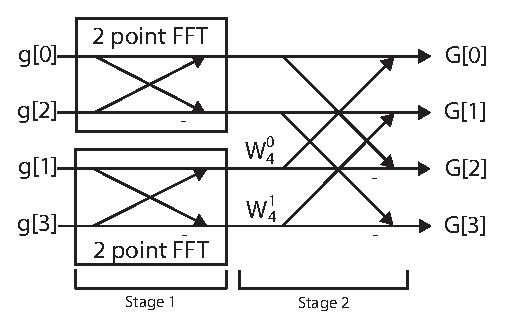
\includegraphics[width=  .5 \textwidth]{images/4ptFFT}
\caption{A four point \gls{fft} divided into two stages. Stage 1 has uses two 2 point \gls{fft}s -- one 2 point \gls{fft} for the even input values and the other 2 point \gls{fft} for the odd input values. Stage 2 performs the remaining operations to complete the \gls{fft} computation as detailed in Equation \ref{eq:reduced4point}. }
\label{fig:4ptFFT}
\end{figure}

Figure \ref{fig:4ptFFT} shows the butterfly diagram for the 4-point \gls{fft}. We can see that the first stage is two 2-point \gls{fft} operations performed on the even (top butterfly) and odd (bottom butterfly) input values. The odd 2-point \gls{fft}s output is multiplied by the appropriate twiddle factor. We can use two twiddle factors for all four output terms using the reduction shown in Equation \ref{eq:reduced4point}.

We are seeing the beginning of a trend that allows the reduction in complexity from $\mathcal{O}(n^2)$ operations for the \gls{dft} to $\mathcal{O}(n \log n)$ operations for the \gls{fft}. The key idea is building the computation through recursion. The 4-point \gls{fft} uses two 2-point \gls{fft}s. This extends to larger \gls{fft} sizes. For example, an 8-point \gls{fft} uses two 4-point \gls{fft}s, which in turn each use two 2-point \gls{fft}s (for a total of four 2-point \gls{fft}s). A 16-point \gls{fft} uses two 8-point \gls{fft}s, and so on.

\begin{exercise}
How many 2 point \gls{fft}s are used in a 32 point \gls{fft}? How many are there in a 64-point \gls{fft}? How many 4 point \gls{fft}s are required for a 64 point \gls{fft}? How about a 128 point \gls{fft}?  What is the general formula for 2-point, 4-point, and 8-point \gls{fft}s in an $N$ point \gls{fft} (where $N > 8$)?
\end{exercise}

Now, let us formally derive the relationship, which provides a general way to describe the recursive structure of the \gls{fft}.  Assume we are calculating an $N$ point \gls{fft}. The formula for calculating the frequency domain values $G[]$ given the input values $g[]$ is:
\begin{equation}
G[k] = \displaystyle\sum\limits_{n=0}^{N-1} g[n] \cdot e^{\frac{-j 2 \pi k n}{N}} \text{ for } k = 0,\dots, N-1
\label{eq:fft-full}
\end{equation}

We can divide this equation into two parts: one that sums the even components and one that sums the odd components.
\begin{equation}
G[k] = \displaystyle\sum\limits_{n=0}^{N/2-1} g[2n] \cdot e^{\frac{-j 2 \pi k (2n)}{N}} + \displaystyle\sum\limits_{n=0}^{N/2-1} g[2n+1] \cdot e^{\frac{-j 2 \pi k (2n+1)}{N}}
\label{eq:fft-split}
\end{equation}
The first part of this equation deals with the even inputs, hence the $2n$ terms in both $g[]$ and in the exponent of $e$. The second part corresponds to the odd inputs with $2n +1$ in both places. Also, note that the sums now go to $N/2 -1$ in both cases, which should make sense since we have divided them into two halves. 

We transform Equation \ref{eq:fft-split} to the following:
\begin{equation}
G[k] = \displaystyle\sum\limits_{n=0}^{N/2-1} g[2n] \cdot e^{\frac{-j 2 \pi k n}{N/2}} + \displaystyle\sum\limits_{n=0}^{N/2-1} g[2n+1] \cdot e^{\frac{-j 2 \pi k (2n)}{N}} \cdot e^{\frac{-j 2 \pi k}{N}}
\label{eq:fft-split-2}
\end{equation}
In the first summation (even inputs), we move the $2$ into the denominator so that it is now $N/2$. The second summation (odd inputs) uses the power rule to separate the $+1$, leaving two complex exponentials. We can further modify this equation to
\begin{equation}
G[k] = \displaystyle\sum\limits_{n=0}^{N/2-1} g[2n] \cdot e^{\frac{-j 2 \pi k n}{N/2}} + e^{\frac{-j 2 \pi k}{N}} \cdot \displaystyle\sum\limits_{n=0}^{N/2-1} g[2n+1] \cdot e^{\frac{-j 2 \pi k n}{N/2}} 
\label{eq:fft-split-3}
\end{equation}
Here, we only modify the second summation. First, we pull one of the complex exponentials outside the summation since it does not depend upon $n$. And we also move the $2$ into the denominator as we did before in the first summation. Note that both summations now have the same complex exponential $e^{\frac{-j 2 \pi k n}{N/2}}$. Finally, we simplify this to 
\begin{equation}
G[k] = A_k + W_N^k B_k 
\label{eq:fft-split-4}
\end{equation} where $A_k$ and $B_k$ are the first and second summations, respectively. And recall that $W = e^{-j 2 \pi}$. This describes an N point \gls{fft} by separating even and odd terms into two summations.

For reasons that will become clear soon, let us assume that we only want to use Equation \ref{eq:fft-split-4} to calculate the first $N/2$ terms, i.e., $G[0]$ through $G[N/2 -1]$. We will derive the remaining $N/2$ terms, i.e., those from $G[N/2]$ to $G[N-1]$ using a different equation. While this may seem counterintuitive or even foolish (why do more math than necessary?), you will see that this will allow us to take advantage of even more symmetry and derive a pattern as we have seen in the 4 point \gls{fft}.

To calculate the higher frequencies $G[N/2]$ to $G[N-1]$, let us derive the same equations but this time using $k = N/2, N/2 + 1, \dots, N -1$.  Thus, we wish to calculate
\begin{equation}
G[k + N/2] = \displaystyle\sum\limits_{n=0}^{N-1} g[n] \cdot e^{\frac{-j 2 \pi (k + N/2) n}{N}} \text{ for } k = 0, \dots, N/2 - 1
\label{eq:fft-upper}
\end{equation}
This is similar to Equation \ref{eq:fft-full} with different indices, i.e., we replace $k$ from Equation \ref{eq:fft-full} with $k + N/2$. Using the same set of transformations that we did previously, we can move directly to the equivalent to Equation \ref{eq:fft-split-3}, but replacing all instances of $k$ with $k + N/2$ which yields 
\begin{equation}
G[k + N/2] = \displaystyle\sum\limits_{n=0}^{N/2-1} g[2n] \cdot e^{\frac{-j 2 \pi (k + N/2) n}{N/2}} + e^{\frac{-j 2 \pi (k + N/2)}{N}} \cdot \displaystyle\sum\limits_{n=0}^{N/2-1} g[2n+1] \cdot e^{\frac{-j 2 \pi (k + N/2) n}{N/2}} 
\label{eq:fft-split-3-upper}
\end{equation}

We can reduce the complex exponential in the summations as follows:
\begin{equation}
e^{\frac{-j 2 \pi (k + N/2) n}{N/2}} = e^{\frac{-j 2 \pi k n}{N/2}} \cdot e^{\frac{-j 2 \pi (N/2) n}{N/2}} = e^{\frac{-j 2 \pi k n}{N/2}} \cdot e^{-j 2 \pi n} = e^{\frac{-j 2 \pi k n}{N/2}} \cdot 1
\label{eq:fft-split-4-upper}
\end{equation}
The first reduction uses the power rule to split the exponential. The second reduction cancels the term $N/2$ in the second exponential. The final reduction uses that fact that $n$ is a non-negative integer, and thus $e^{-j 2 \pi n}$ will always be a rotation of multiple of $2 \pi$. This means that this term is always equal to $1$. 

Now let us tackle the second complex exponential
\begin{equation}
e^{\frac{-j 2 \pi (k + N/2)}{N}} = e^{\frac{-j 2 \pi k }{N}} \cdot e^{\frac{-j 2 \pi N/2 }{N}} = e^{\frac{-j 2 \pi k }{N}} \cdot e^{-j  \pi} = - e^{\frac{-j 2 \pi k }{N}}
\label{eq:fft-split-5-upper}
\end{equation}
The first reduction splits the exponential using the power rule. The second reduction does some simplifications on the second exponential. We get the final term by realizing that $e^{-j \pi} = -1$.

By substituting Equations \ref{eq:fft-split-4-upper} and \ref{eq:fft-split-5-upper} into Equation \ref{eq:fft-split-3-upper}, we get
\begin{equation}
G[k + N/2] = \displaystyle\sum\limits_{n=0}^{N/2-1} g[2n] \cdot e^{\frac{-j 2 \pi k n}{N/2}} - e^{\frac{-j 2 \pi k}{N}} \cdot \displaystyle\sum\limits_{n=0}^{N/2-1} g[2n+1] \cdot e^{\frac{-j 2 \pi k n}{N/2}} 
\label{eq:fft-split-6-upper}
\end{equation}
Note the similarity to Equation \ref{eq:fft-split-3}. We can put it in terms of Equation \ref{eq:fft-split-4} as
\begin{equation}
G[k + N/2] = A_k - W_N^k B_k 
\label{eq:fft-split-7-upper}
\end{equation}

We can use Equations \ref{eq:fft-split-4} and \ref{eq:fft-split-7-upper} to create an $N$ point \gls{fft} from two $N/2$ point \gls{fft}s. Remember that $A_k$ corresponds to the even input values, and $B_k$ is a function of the odd input values. Equation \ref{eq:fft-split-4} covers the first $N/2$ terms, and Equation \ref{eq:fft-split-7-upper} corresponds to the higher $N/2$ frequencies. 

\begin{figure}
\centering
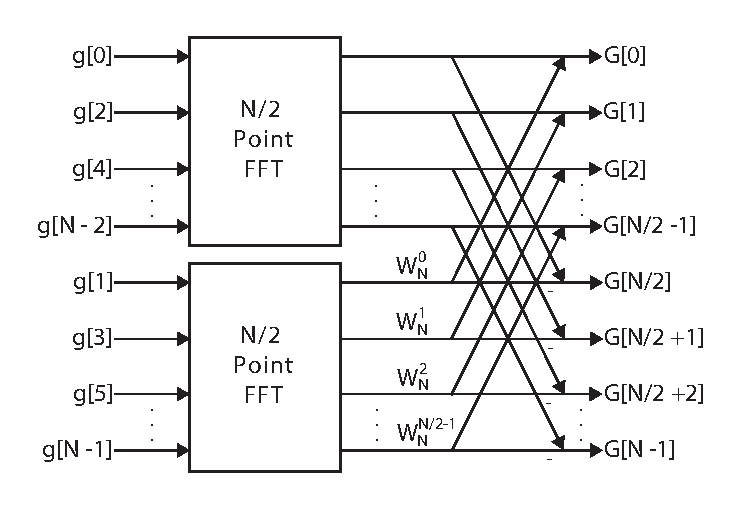
\includegraphics[width=  .8 \textwidth]{images/NptFFT}
\caption{Building an $N$ point \gls{fft} from two $N/2$ point \gls{fft}s. The upper $N/2$ point \gls{fft} is performed on the even inputs; the lower $N/2$ \gls{fft} uses the odd inputs. }
\label{fig:NptFFT}
\end{figure}

Figure \ref{fig:NptFFT} shows an $N$ point \gls{fft} derived from two $N/2$ point \gls{fft}s. $A_k$ corresponds to the top $N/2$ \gls{fft}, and $B_k$ is the bottom $N/2$ \gls{fft}.  The output terms $G[0]$ through $G[N/2-1]$ are multiplied by $W_N^0$ while the output terms $G[N/2]$ through $G[N-1]$ are multiplied by $-W_N^0$. Note that the inputs $g[]$ are divided into even and odd elements feeding into the top and bottom $n/2$ point \gls{fft}s, respectively.

We can use the general formula for creating the \gls{fft} that was just derived to recursively create the $N/2$ point \gls{fft}. Each of the $N/2$ point \gls{fft}s can be implemented using two $N/4$ point \gls{fft}s. And each $N/4$ point \gls{fft} uses two $N/8$ point \gls{fft}s, and so on, until we reach the base case, a 2-point \gls{fft}.

Figure \ref{fig:8ptFFT} shows an 8-point \gls{fft} and highlights this recursive structure. The boxes with the dotted lines indicate different sizes of \gls{fft}. The outermost box indicates an 8-point \gls{fft}. This is composed of two 4-point \gls{fft}s. Each of these 4-point \gls{fft}s has two 2-point \gls{fft}s for a total of four 2-point \gls{fft}s. 

\begin{figure}
\centering
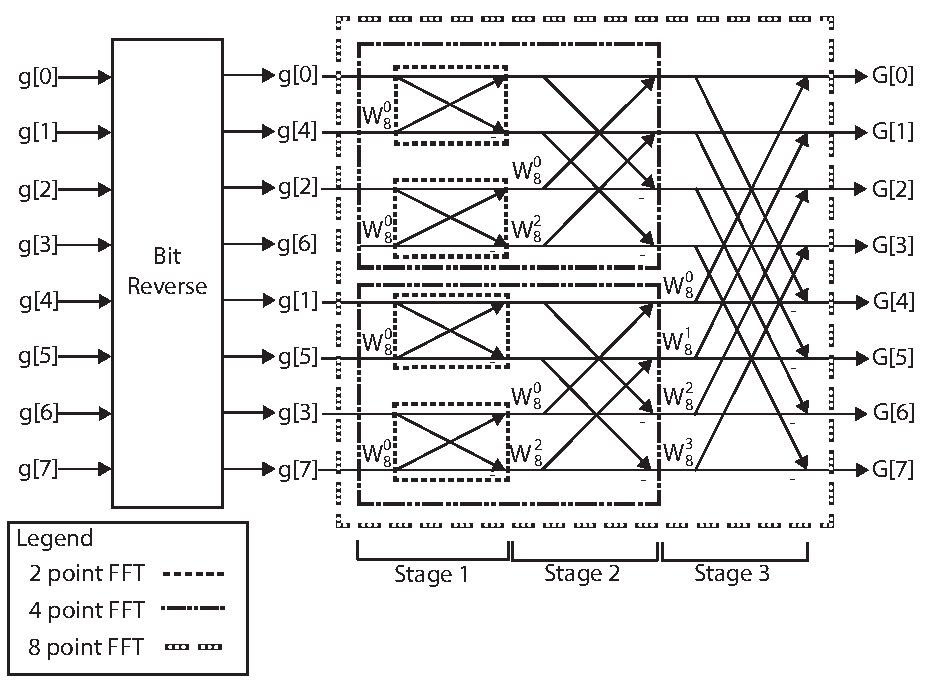
\includegraphics[width=  \textwidth]{images/8ptFFT}
\caption{An 8 point \gls{fft} built recursively. There are two 4-point \gls{fft}s, each using two 2-point \gls{fft}s. The inputs must be reordered to even and odd elements twice. This results in reordering based on the bit reversal of the indices.}
\label{fig:8ptFFT}
\end{figure}

Also, the inputs must be reordered before being fed into the 8-point \gls{fft} because the different $N/2$ point \gls{fft}s take even and odd inputs. The upper four inputs correspond to even inputs, and the lower four inputs have odd indices. However, they are reordered twice. If we separate the even and odd inputs once we have the even set $\{g[0], g[2], g[4], g[6] \}$ and the odd set $\{g[1], g[3], g[5], g[7] \}$. Now let us reorder the even set once again. In the even set $g[0]$ and $g[4]$ are the even elements, and $g[2]$ and $g[6]$ are the odd elements. Thus reordering it results in the set $\{g[0], g[4], g[2], g[6] \}$. The same can be done for the initial odd set yielding the reordered set $\{g[1], g[5], g[3], g[7] \}$. 

The final reordering is done by swapping values whose indices are in a bit reversed order. Table \ref{table:bit_reverse} shows the indices and their three-bit binary values. The table shows the eight indices for the 8 point \gls{fft} and the corresponding binary value for each of those indices in the second column. The third column is the bit-reversed binary value of the second column. The last column is the decimal number corresponding to the reversed binary number. 

\begin{table}[htbp]
\caption{The index, three-bit binary value for that index, bit reversed binary value, and the resulting bit reversed index.}
\begin{center}
\begin{tabular}{|c|c|c|c|}
\hline
Index & Binary & Reversed & Reversed \\
 & & Binary & Index \\
\hline
0 & 000 & 000 & 0 \\
1 & 001 & 100 & 4 \\
2 & 010 & 010 & 2 \\
3 & 011 & 110 & 6 \\
4 & 100 & 001 & 1 \\
5 & 101 & 101 & 5 \\
6 & 110 & 011 & 3 \\
7 & 111 & 111 & 7 \\
\hline
\end{tabular}
\end{center}
\label{table:bit_reverse}
\end{table}

Looking at the first row, the initial index $0$ has a binary value of $000$, which, when reversed, remains $000$. Thus, this index does not need to be swapped. Looking at Figure \ref{fig:8ptFFT}, we see this is true. $g[0]$ remains in the same location. In the second row, the index 1 has a binary value $001$. When reversed, this is $100$ or $4$. Thus, the data that initially started at index 1, i.e., $g[1]$, should end up in the fourth location. Looking at index 4, we see that the bit reversed value is $1$. Thus $g[1]$ and $g[4]$ are swapped.  

This bit reversal process works regardless of the input size of the \gls{fft}, assuming that the \gls{fft} is a power of two. \gls{fft} are commonly a power of two since this allows them to be recursively implemented.

\begin{exercise}
In a 32 point \gls{fft}, index 1 is swapped with which index? Which index is index 2 is swapped with?
\end{exercise}

This completes our mathematical treatment of the \gls{fft}. There are plenty of more details about the \gls{fft} and how to optimize it. We may have spent too much time already discussing the finer details of the \gls{fft}; this is a book on parallel programming for FPGAs, not digital signal processing. This highlights an integral part of creating an optimum hardware implementation -- the designer must understand the algorithm under development. Without that, it isn't easy to create an optimized implementation. The following section deals with creating a good \gls{fft} implementation. 

\section{Baseline Implementation}

In the remainder of this chapter, we discuss different methods to implement the Cooley-Tukey \gls{fft} \cite{cooley65} algorithm using the \VHLS tool. This is the same algorithm that we described in the previous section. We start with a standard version of the code and then describe how to restructure it to achieve a better hardware design. 

When performed sequentially, the $\mathcal{O}(n \log n)$ operations in the \gls{fft} require $\mathcal{O}(n \log n)$ time steps.   A parallel implementation will perform some portion of the \gls{fft} in parallel.  One common way of parallelizing the \gls{fft} is to organize the computation into $\log n$ stages, as shown in Figure \ref{fig:fftstages}.  The operations in each stage depend on the previous stage's operations, naturally leading to a pipelining across the tasks.  Such an architecture allows $\log n$ \glspl{fft} to be computed simultaneously with a task interval determined by the architecture of each stage.  We discuss task pipelining using the \lstinline|dataflow| directive in Section \ref{sec:fft_task_pipelining}.

Each stage in the \gls{fft} also contains significant parallelism since each butterfly computation is independent of other butterfly computations in the same stage.  In the limit, performing $n/2$ butterfly computations every clock cycle with a Task Interval of 1 can allow the entire stage to be computed with a Task Interval of 1.  The parallelism in the \gls{fft} algorithm can be exploited when combined with a dataflow architecture.  Note, however, that although such an architecture can be constructed, it is seldom used except for very small signals since an entire new block of \lstinline|SIZE| samples must be provided every clock cycle to keep the pipeline fully utilized.  For instance, a 1024-point \gls{fft} of complex 32-bit floating point values, running at 250 MHz would require 1024 \text{points}*(8 {bytes}/{point})*250*$10^9$ Hz = 1Terabyte/second of data into the FPGA.   A designer must match the computation architecture to the system's required data rate.

\begin{exercise}
Assuming a clock rate of 250 MHz and one sample received every clock cycle, approximately how many butterfly computations must be implemented to process every sample with a 1024-point \gls{fft}?  What about for a 16384-point \gls{fft}?
\end{exercise}

In the remainder of this section, we describe the optimization of an \gls{fft} with the function prototype \lstinline|void fft(DTYPE X_R[SIZE], DTYPE X_I[SIZE])| where \lstinline|DTYPE| is a user-customizable data type for the representation of the input data. This may be \lstinline|int|, \lstinline|float|, or a fixed point type. For example, \lstinline|#define DTYPE int| defines \lstinline|DTYPE| as an \lstinline|int|. Note that we choose to implement the real and imaginary parts of the complex numbers in two separate arrays. The \lstinline|X_R| array holds the real input values, and the \lstinline|X_I| array holds the imaginary values. \lstinline|X_R[i]| and \lstinline|X_I[i]| hold the $i$th complex number in separate real and imaginary parts. 

\begin{aside}
In this section, we describe one change in the \gls{fft} implementation. Here, we perform an \gls{fft} on complex numbers. The previous section uses only real numbers. While this may seem like a major change, the core ideas remain unchanged. The only differences are that the data has two values (corresponding to the real and imaginary part of the complex number), and the operations (add, multiply, etc.) are complex operations. 
\end{aside}

This function prototype forces an in-place implementation. The output data is stored in the same array as the input data. This eliminates the need for additional arrays for the output data, reducing the memory required for the implementation. However, this may limit the performance since we must read the input data and write the output data to the same arrays. Using separate arrays for the output data is reasonable if it can increase the performance. There is always a tradeoff between resource usage and performance; the same is true here. The best implementation depends upon the application requirements (e.g., high throughput, low power, size of FPGA, size of the \gls{fft}, etc.).

%\section{Initial ``Software'' \gls{fft} Implementation}

We start with code for an \gls{fft} that would be typical for a software implementation. Figure \ref{fig:fft_sw} shows a nested three \lstinline|for| loop structure. The outer \lstinline|for| loop, labeled \lstinline|stage_loop| implements one stage of the \gls{fft} during each iteration. There are $log_2(N)$ stages where $N$ is the number of input samples. The stages are clearly labeled in Figure \ref{fig:8ptFFT}; this 8 point \gls{fft} has $log_2(8) = 3$ stages. You can see that each stage performs the same amount of computation or the same number of butterfly operations. Each stage has four butterfly operations in the 8-point \gls{fft}. 

\begin{figure}
\lstinputlisting[format=none,firstline=34]{examples/fft_sw.cpp}
\caption{ A common implementation for the \gls{fft} using three nested \lstinline|for| loops.  While this may work well running as software on a processor, it is far from optimal for a hardware implementation.}
\label{fig:fft_sw}
\end{figure}

\begin{exercise}
How many butterfly operations exist in each stage for an $N$-point \gls{fft}? How many total butterfly operations exist for the entire \gls{fft}?
\end{exercise}

The second \lstinline|for| loop, labeled \lstinline|butterfly_loop|, performs all butterfly operations for the current stage. \lstinline|butterfly_loop| has another nested \lstinline|for| loop, labeled \lstinline|dft_loop|. Each iteration of \lstinline|dft_loop| performs one butterfly operation. Remember that we are dealing with complex numbers and must perform complex additions and multiplications. 

The first line in \lstinline|dft_loop| determines the offset of the butterfly. Note that the ``width'' of the butterfly operations changes depending upon the stage. Looking at Figure \ref{fig:8ptFFT}, Stage 1 performs butterfly operations on adjacent elements, Stage 2 performs butterfly operations on elements with index differing by two, and Stage 3 performs butterfly operations on elements with index differing by four. This difference is computed and stored in the \lstinline|i_lower| variable. Notice that this offset, stored in the variable \lstinline|numBF|, differs in every stage. 

The remaining operations in \lstinline|dft_loop| perform multiplication by the twiddle factor and an addition or subtraction operation. The variables \lstinline|temp_R| and \lstinline|temp_I| hold the real and imaginary portions of the data after multiplication by the twiddle factor $W$. The variables \lstinline|c| and \lstinline|s| are $ W$'s real and imaginary parts, calculated using the \lstinline|sin()| and \lstinline|cos()| built-in functions. We could also use the CORDIC, such as the one developed in Chapter \ref{chapter:cordic}, to have more control over the implementation. Twiddle factors are also commonly precomputed and stored in on-chip memory for moderate array sizes.  Lastly, elements of the \lstinline|X_R[]| and \lstinline|X_I[]| arrays are updated with the result of the butterfly computation.

\lstinline|dft_loop| and \lstinline|butterfly_loop| each executes a different number of times depending upon the stage. However, the total number of times the body of \lstinline|dft_loop| is executed in one stage is constant. The number of iterations for the \lstinline|butterfly for| loop depends upon the number of unique $W$ twiddle factors in that stage. Referring again to Figure \ref{fig:8ptFFT}, we can see that Stage 1 uses only one twiddle factor, in this case $W_8^0$. Stage 2 uses two unique twiddle factors, and Stage 3 uses four different $W$ values. Thus, \lstinline|butterfly_loop| has only one iteration in Stage 1, 2 iterations in Stage 2, and four iterations in Stage 3. Similarly, the number of iterations of \lstinline|dft_loop| changes. It iterates four times for an 8-point \gls{fft} in Stage 1, two times in Stage 2, and only once in Stage 3. However, in every stage, the body of \lstinline|dft_loop| is executed the same number of times, performing four butterfly operations for each stage of an 8-point \gls{fft}. 

\begin{aside}
\VHLS performs significant static analysis on each synthesized function, including computing bounds on the number of times each loop can execute.  This information comes from many sources, including variable bitwidths, ranges, and \lstinline|assert()| functions in the code. When combined with the loop II, \VHLS can compute bounds on the latency or interval of the \gls{fft} function.  In some cases (usually when loop bounds are variable or contain conditional constructs), the tool cannot compute the latency or interval of the code and returns `'?'.  When synthesizing the code in Figure \ref{fig:fft_sw}, \VHLS may not be able to determine the number of times that \lstinline|butterfly_loop| and \lstinline|dft_loop| iterate because these loops have variable bounds.

The \lstinline|tripcount| directive enables the user to specify to the \VHLS tool more information about the number of times a loop is executed, which can be used by the tool to analyze the design performance. It takes three optional arguments: \lstinline|min|, \lstinline|max|, and \lstinline|average|. This code could add a directive to \lstinline|dft_loop|. By applying this directive, the \VHLS tool can calculate bounds on the latency and interval value for the loop and the overall design.  Note that since the \VHLS tool uses the numbers you provide, if you give the tool an incorrect tripcount, the reported task latency and task interval will be incorrect -- garbage in, garbage out.   
\end{aside}

\begin{exercise}
What is the appropriate way to use the \lstinline|trip count| directive for the \gls{fft} in Figure \ref{fig:fft_sw}? Should you set the \lstinline|max|, \lstinline|min|, and/or \lstinline|average| arguments? Would you need to modify the tripcount arguments if the size of the \gls{fft} changes?  
\end{exercise}

\section{Bit Reversal}
\label{sec:fft_bit_reversal}

We have not discussed the bit reverse function, which swaps the input data values to perform an in-place \gls{fft}. This means that the input values are mixed, resulting in the output data being in the correct order. We discuss that function in some detail now.

Figure \ref{fig:fft_bit_reverse} shows one possible implementation of the bit reverse function. It divides the code into two functions. The first is the bit reversal function (\lstinline|bit_reverse|), which reorders data in the given arrays so that each data is located at a different index in the array. This function calls another function, \lstinline|reverse_bits|, which takes an input integer and returns the bit-reversed value of that input.

\begin{figure}
\lstinputlisting[lastline=33]{examples/fft_sw.cpp}
\caption{ The first stage in our \gls{fft} implementation reorders the input data. This is done by swapping the value at index $i$ in the input array with the value at the bit-reversed index corresponding to $i$. The function \lstinline|reverse_bits| gives the bit reversed value corresponding to the \lstinline|input| argument. The function \lstinline|bit_reverse| swaps the values in the input array. }
\label{fig:fft_bit_reverse}
\end{figure}

Let us start with a brief overview of the \lstinline|reverse_bits| function. The function goes bit by bit through the \lstinline|input| variable and shifts it into the \lstinline|rev| variable. The \lstinline|for| loop body consists of a few bitwise operations that reorder the input bits. Although these operations are individually not terribly complex, the intention of this code is that the for loop is completely unrolled, and \VHLS can identify that the bits of the input can be wired to the output.  As a result, implementing the \lstinline|reverse_bits| function should require no logic resources but only wires.  This is a case where unrolling loops greatly simplifies the operations that must be performed.  The individual `or' operations must be performed sequentially without unrolling the loop.  Although this loop can be pipelined, the `or' operation would still be implemented in logic resources in the FPGA, and executing the loop would have a latency determined by the number of bits being reversed (\lstinline|\gls{fft}_BITS| in this case).

\begin{exercise}
What is the latency of the \lstinline|reverse_bits| function when no directives are applied? What is the latency when the loop is pipelined?  What is the latency when the whole function is pipelined?
\end{exercise}

\begin{aside}
It is tempting to ``blindly'' apply directives to achieve a better design. However, this can be counterproductive. The best designer deeply understands both the application and the available optimizations and carefully considers these together to achieve the best results. 
\end{aside}

Now, let us optimize the parent \lstinline|bit_reverse| function. This function has a single \lstinline{for} loop that iterates through each index of the input arrays. Note that there are two input arrays \lstinline{X_R[]} and \lstinline{X_I[]}. Since we are dealing with complex numbers, we must store both the real portion (in the array \lstinline{X_R[]}) and the imaginary portion (in the array \lstinline{X_I[]}). \lstinline{X_R[i]} and \lstinline{X_I[i]} hold the real and imaginary values of the i-th input.
In each iteration of the \lstinline{for} loop, we find the index reversed value by calling the \lstinline{reverse_bits} function. Then we swap both the real and imaginary values stored in the index \lstinline{i} and the index returned by the function \lstinline{reverse_bits}. We will eventually hit the reversed index for every value as we go through all \lstinline{SIZE} indices. Thus, the code only swaps values the first time based on the condition \lstinline{if(i < reversed)}.

%To me this doesn't say much that this point...  it would be better to discuss this in a case where it really matters
%We can optimize this function in a number of different ways. Since the \lstinline{reverse_bits} function is small and efficient, it make sense to use the \lstinline{inline} pragma. This essentially copies all of the code from within the \lstinline{reverse_bits} function directly into the \lstinline{bit_reverse} function. Thus there is no function call, and any overhead associated with it goes away. Furthermore, this allows the \VHLS tool to optimize the code within the \lstinline{reverse_bits} function along with the code in the \lstinline{bit_reverse} function, which can lead to some additional efficiencies. That being said, it may be the case when the \lstinline{inline} directive does not help. 

\section{Task Pipelining}
\label{sec:fft_task_pipelining}

Dividing the \gls{fft} algorithm into stages enables \VHLS to generate an implementation where different stages of the algorithm are operating on different data sets. This optimization, called \gls{taskpipelining}, is enabled using the \lstinline{dataflow} directive. This is a common hardware optimization and, thus, is relevant across a range of applications.

\begin{figure}
\lstinputlisting[format=none,firstline=35]{examples/fft_stages.cpp}
\caption{Code implementing an 8 point \gls{fft} divided into stages, each implemented by a separate function. The \lstinline{bit_reverse} function is the first stage. Each following stage implements butterfly operations. }
\label{fig:fft_stages_code}
\end{figure}

We can naturally divide the \gls{fft} algorithm into $\log_2(N+1)$ stages where $N$ is the number of points of the \gls{fft}.  The first stage swaps each element in the input array with the element located at the bit-reversed address in the array. After this bit reverse stage, we perform $\log_2(N)$ stages of butterfly operations. Each of these butterfly stages has the same computational complexity.  Figure \ref{fig:fft_stages_code} describes dividing an 8-point \gls{fft} into four separate tasks. The code has separate function calls for each task: one call to \lstinline{bit_reverse} and three calls to \lstinline{fft_stage}. Each stage has two input arrays and two output arrays: one for the real portion and one for the imaginary portion of the complex numbers. Assume that the \lstinline{DTYPE} is defined elsewhere, e.g., as an \lstinline{int}, \lstinline{float} or a fixed point data type.

Refactoring the \gls{fft} code allows us to perform \gls{taskpipelining}. Figure \ref{fig:fftstages} gives an example of this. In this execution, rather than wait for the first task to complete all four function calls in the code before the second task can begin, the second task can start after the first task has only completed the first function \lstinline{bit_reverse}. The first task continues to execute each stage in the pipeline in order, followed by the remaining tasks in order.  Once the pipeline is full, all four subfunctions are executed concurrently, but each operates on different input data. Similarly, there are four 8-point \glspl{fft} being computed simultaneously, each one executing on a different component of the hardware. This is shown in the middle portion of Figure \ref{fig:fftstages}. Each of the vertical four stages represents one 8-point \gls{fft}. And the horizontal denotes increasing time. Thus, once we start the fourth 8 point \gls{fft}, we have four \glspl{fft} running simultaneously.  Note that for this to work, each call to the \lstinline{fft_stage} function must be implemented with independent hardware.  In addition, enough storage is required to contain the intermediate computations of each \gls{fft} being computed simultaneously.

\begin{figure}
\centering
%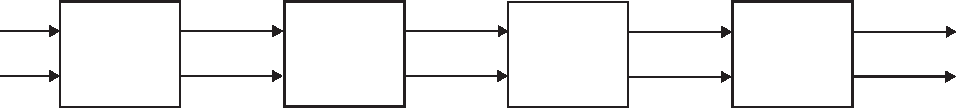
\includegraphics[width=  \textwidth]{images/fftstages}
{\scriptsize \includesvg{fftstages}}
\includesvg{fft_dataflow_behavior}
\caption{ Dividing the \gls{fft} into different stages allows for task pipelining across each stage. The figure shows an example with three \gls{fft} stages (i.e., an 8 point \gls{fft}). The figure shows four 8-point \gls{fft} executing simultaneously. }
\label{fig:fftstages}
\end{figure}

The \lstinline|dataflow| directive can construct separate pipeline stages (often called \glspl{process}) from functions and loops. The code in Figure \ref{fig:fft_stages_code} uses functions only, but we could achieve a similar result with four loops instead of four functions.  This result could be achieved by explicitly unrolling the outer \lstinline|stage_loop| in the original code or using \lstinline|#pragma HLS unroll|.  Such a code structure has several advantages.  Firstly, it is closer to the original algorithmic code's structure, reducing the number of code changes that need to be made.   Secondly, the code is less verbose, making it somewhat easier to write.  Thirdly, the code is parameterized again, supporting values of different sizes with the same code.  Code with a loop is shown in Figure \ref{fig:fft_stages_loop_code}.

\begin{figure}
\lstinputlisting[format=none,firstline=64]{examples/fft_stages_loop.cpp}
\caption{Code implementing an arbitrary-sized FFT using a loop. After the loop is unrolled, each function call in the unrolled loop becomes a dataflow process. }
\label{fig:fft_stages_loop_code}
\end{figure}

The \lstinline{dataflow} directive and the \lstinline{pipeline} directive generate circuits capable of pipelined execution.  The key difference is in the granularity of the pipeline. The \lstinline{pipeline} directive constructs an architecture that is efficiently pipelined at the cycle level and is characterized by the II of the pipeline.  Operators are statically scheduled; if the II is greater than one, operations can be shared on the same operator.  The \lstinline{dataflow} directive constructs an architecture that is efficiently pipelined for operations that take a (possibly unknown) number of clock cycles, such as the behavior of a loop operating on a block of data.  These coarse-grained operations are not statically scheduled, and the behavior is controlled dynamically by the handshake of data through the pipeline.  In the case of the \gls{fft}, each stage is an operation on a block of data (the whole array), which takes a large number of cycles.  Within each stage, loops execute individual operations on the data in a block.  Hence, this is a case where it often makes sense to use the \lstinline|dataflow| directive at the top level to form a coarse-grained pipeline, combined with the \lstinline|pipeline| directive within each loop to form fine-grained pipelines of the operations on each data element.

The \lstinline{dataflow} directive must implement memories to pass data between different processes. When \VHLS can determine that processes access data in sequential order, it implements the memory using a FIFO. This requires that data is written into an array in the same order that it is read from the array.  If this is not the case, or if \VHLS can not determine if this streaming condition is met, then the memory can be implemented using a ping-pong buffer instead.   The ping-pong buffer consists of two (or more) conceptual blocks of data, each the size of the original array. One of the blocks can be written by the source process while the destination process reads the other block. The term ``ping-pong'' comes from the fact that the reading and writing to each block of data alternates in every task execution. The source process will write to one block and then switch to the other before beginning the next task. The destination process reads from the block the producer is not writing to. As a result, the source and destination processes never write and read from the same block simultaneously. 

A ping-pong buffer requires enough memory to store each communication array at least twice.   FIFOs can often be significantly smaller, but determining a minimal size for each FIFO is often difficult to reason about.  Unlike a FIFO, however, the data in a ping-pong buffer can be written to and read from in any order. Thus, FIFOs are generally the best choice when the data is produced and consumed in sequential order, and ping-pong buffers are a better choice when there are no such regular data access patterns.

Using the \lstinline{dataflow} directive effectively still requires optimizing each process's behavior. Each process in the pipeline can still be optimized using techniques we have seen previously, such as code restructuring, pipelining, and unrolling.  For example, we have already discussed optimizations for the \lstinline{bit_reverse} function in Section \ref{sec:fft_bit_reversal}.  In general, it is important to optimize individual tasks while considering overall performance goals. It is often best to start with small functions and understand how to optimize them in isolation. As a designer, comprehending what happens in a small piece of code and hopefully determining the best optimizations quickly is often easier. After optimizing each function, you can move up the hierarchy by considering larger functions, given particular implementations of low-level functions, eventually reaching the top-level function.

However, the local optimizations must be considered in the overall scope of the goals. In particular, for dataflow designs, the achieved interval for the overall pipeline can never be smaller than the interval of each process. Looking again at Figure \ref{fig:fft_stages_code}, assume that \lstinline{bit_reverse} has an interval of 8 cycles, \lstinline{fft_stage(1,...)} has an interval of 12 cycles, \lstinline{fft_stage(2,...)} has an interval of 12 cycles, and \lstinline{fft_stage(3,...)} has an interval of 14 cycles. When using \lstinline{dataflow}, the overall task interval is 14, determined by the maximum of all tasks/functions. This means that you should be careful in balancing optimizations across different processes to create a balanced pipeline where the interval of each process is approximately the same. In this example, improving the interval of the \lstinline{bit_reverse} function cannot improve the overall interval of the \lstinline|fft| function. Increasing the latency of the \lstinline{bit_reverse} function might be beneficial if it can be achieved with significantly fewer resources.

\section{Conclusion}
\label{sec:fft_conclusion}

The overall goal is to create the most optimal design, which is a function of your application's needs. This may be to create the smallest implementation. The goal could be creating something that can perform the highest throughput implementation regardless of the size of the FPGA or the power/energy constraints. The latency of delivering the results may matter if the application has real-time constraints. All of the optimizations change these factors in different ways. 

In general, there is no one algorithm for optimizing your design. It is a complex function of the application, design constraints, and the designer's inherent abilities. Yet, it is important that the designer have a deep understanding of the application, the design constraints, and the abilities of the synthesis tool. 

We attempted to illustrate these bits of wisdom in this chapter. While the \gls{fft} is a well-studied algorithm with many known hardware implementation tricks, it still serves as a good exemplar for high-level synthesis. We did not give all of the tricks for optimization. %e leave that as an exercise in Chapter \ref{chapter:ofdm} where we task the designer to create an simple orthogonal frequency-division multiplexing receiver. The core of this an \gls{fft}.  
Regardless, we provided some insight into the key optimizations here, which we hope serve as a guide to how to optimize the \gls{fft} using the \VHLS tool.

First and foremost, understand the algorithm. We spent a lot of time explaining the basics of the \gls{fft}, and how it relates to the \gls{dft}. We hope the reader understands this is the most important part of building optimal hardware. Indeed, the designer could translate C/MATLAB/Java/Python code into \VHLS and get a working implementation. And that same designer could blindly apply directives to achieve better results. However, that designer will not get anywhere close to optimal results without a deep understanding of the algorithm itself.

Second, we introduce  task-level pipelining using the \lstinline{dataflow} directive. This is a powerful optimization that is not possible through code restructuring. I.e., the designer must use this optimization to get such a design. Thus, the designer must understand its power, drawbacks, and usage.

Additionally, we build upon some of the optimizations from previous chapters, e.g., loop unrolling and pipelining. All of these are important to get an optimized \gls{fft} hardware design. While we only spent a little bit of time on these optimizations, they are extremely important.

Finally, we tried to convey that these optimizations cannot be done in isolation. Sometimes, the optimizations are independent and can be done in isolation. For example, we can focus on one of the tasks (e.g., in the \lstinline{bit_reverse} function as we did in Section \ref{sec:fft_bit_reversal}). However, many times, different optimizations will affect one another. For example, the \lstinline{inline} directive will affect the way the pipelining of a function. In particular, the way that we optimize tasks/functions can propagate itself up through the hierarchy of functions.  The takeaway is that the designer must understand the effects of the optimizations on the algorithm, both locally and globally.
